\documentclass[11pt,a4paper]{article}

\setlength{\textwidth}{165mm}
\setlength{\textheight}{240mm}
\setlength{\parindent}{0mm} % S{\aa} meget rykkes ind efter afsnit
\setlength{\parskip}{\parsep}
\setlength{\headheight}{0mm}
\setlength{\headsep}{0mm}
\setlength{\hoffset}{-2.5mm}
\setlength{\voffset}{0mm}
\setlength{\footskip}{15mm}
\setlength{\oddsidemargin}{0mm}
\setlength{\topmargin}{0mm}
\setlength{\evensidemargin}{0mm}

\usepackage{courier}
\usepackage{amsmath}
\usepackage[a4paper, hmargin={2.8cm, 2.8cm}, vmargin={2.5cm, 2.5cm}]{geometry}
\usepackage{eso-pic} % \AddToShipoutPicture
\usepackage{graphicx} % \includegraphics
\usepackage[english]{babel}
\usepackage[utf8]{inputenc}
\usepackage{amsfonts,amsmath,amssymb}
\usepackage[colorinlistoftodos]{todonotes}
\usepackage{gauss}
\usepackage{enumitem}
\usepackage{hyperref}
\usepackage{microtype}
\usepackage{listings} %code parsing
\lstset{language=bash} %java code
\newcommand{\code}[1]{\texttt{#1}}

\newlist{SubItemList}{itemize}{1}
\setlist[SubItemList]{label={$-$}}

\let\OldItem\item
\newcommand{\SubItemStart}[1]{%
    \let\item\SubItemEnd
    \begin{SubItemList}[resume]%
        \OldItem #1%
}
\newcommand{\SubItemMiddle}[1]{%
    \OldItem #1%
}
\newcommand{\SubItemEnd}[1]{%
    \end{SubItemList}%
    \let\item\OldItem
    \item #1%
}
\newcommand*{\SubItem}[1]{%
    \let\SubItem\SubItemMiddle%
    \SubItemStart{#1}%
}%

\newcommand{\BAR}{%
  \hspace{-\arraycolsep}%
  \strut\vrule % the `\vrule` is as high and deep as a strut
  \hspace{-\arraycolsep}%
}

\author{\Large{Sven Frenzel \href{mailto:sven@frenzel.dk}{(sven@frenzel.dk)} - 130793 - cdn769 - Hold Passov}\\
\Large{Mads Gram \href{mailto:mgmadsgram@gmail.com}{(mgmadsgram@gmail.com)}  - 081293 - wtc324 - Hold Passov}\\
\Large{Thorkil Værge \href{mailto:thorkilk@gmail.com}{(thorkilk@gmail.com)} - 150287 - wng750 - Hold Passov}}

\title{
\vspace{3cm}
\Large{First Partial Assignment - ProjDat}
}

\begin{document}

%% Change `ku-farve` to `nat-farve` to use SCIENCE's old colors or
%% `natbio-farve` to use SCIENCE's new colors and logo.
\AddToShipoutPicture*{\put(0,0){\includegraphics*[viewport=0 0 700 600]{include/natbio-farve}}}
\AddToShipoutPicture*{\put(0,602){\includegraphics*[viewport=0 600 700 1600]{include/natbio-farve}}}

%% Change `ku-en` to `nat-en` to use the `Faculty of Science` header
\AddToShipoutPicture*{\put(0,0){\includegraphics*{include/nat-en}}}

\clearpage\maketitle
\thispagestyle{empty}

\newpage

\section{Projektdefintion}
\subsection{Problem statement}
\subsubsection{Problem Domain}
At the University, many courses require the students to hand in assignments. In this modern era, this is done by electronic hand-ins over the World Web Web on the interconnected global network. It is essential to ensure that there can be no doubt of the identity of the student handing in the assignment because the teachers grade the students based on these electronic hand-ins. \\\\

This problem can be solved by a classic login system, where the user has a unique username and picks a password as a secret piece of information to avoid malicious parties to get access to user privileges. This system has already been implemented by the Norwegian company its Learning through the World Wide Web platform ``Absalon''.\\\\

Another option, which is the subject of this project, is to use asymmetric key encryption. In this system the user, i.e. the student, generates a key pair on his own computer. This keypair can be used for authentication and can also be used in other situations. The authenticity of the key pair can be further validated by peer-to-peer authentication through the signing of other peoples' keys.\\\\

The students at the University of Copenhagen all have a unique username in the form of a ``KU Username''. If this username is mapped to a public key and the student holds the equivalent private key, then the authentication of an electronic hand-in has the same degree of trusted authenticity as that of the key pair. \\\\

We can use the KU login in order to establish this mapping and this mapping can be further authenticated by the above-mentioned peer-to-peer key signing although this latter authentication is not necessary for the system to work. I.e., support for peer-to-peer signing in this project is nice-to-have, not need-to-have. As a way to establish this mapping, the KU login is used as a trusted source of linking an identity to a public key. The role, if any, of peer-to-peer signing or key signing by teachers has not yet been established.
\subsubsection{Scenarios}
\begin{itemize}
\item A student has just started on the course ``Maskinarkitektur'' (Processor Design). He learns that he has to hand in the assignment by signing it with an OpenPGP key. He must then generate his own key pair using a designated program like ``GPG4Win'' or through a webservice developed as a part of this project and hosted by KU. After the key pair has been generated, the student uploads his public key to a server and the server then stores the KU Username and the public key. 
\item When the student hands in his assignment, he signs it with his newly generated private key. And the signature is then uploaded along with the assignment. A teacher is grading the assignments that has been handed in on the course ``Maskinarkitektur''. Before he grades them, he needs to check the validity of the identity of the student. This check can either be done automatically by software that interfaces with the system developed as part of this project or manually by the teacher.
\item All teachers have their OpenPGP-keys on the service and sign all feedback. These public keys must be available for the students.
\end{itemize}
\subsubsection{Functional Requirements}
\begin{itemize}
\item The system must map a KU Username to a OpenPGP public key.
\item Users must be able to upload their own public key to the service.
\item If a user loses his private key, a method for replacing the public key must exist.
\item The initial registration of a key, and the replacement of a key, is authenticated through the KU email system. 
\item Lookups in this table must be possible for the relevant university staff. An API will be defined and implemented for this.
\item The KU usernames must not be accessible for outsiders.
\item A guide for creating key pairs needs to be available on the website, possibly as shell script. This guide should explain how to derive an SSH key from an OpenPGP key.
\end{itemize}
\subsubsection{Nunfunctional Requirements}
\begin{itemize}
\item The backend should be written in golang.
\item The frontend should be Javascript and/or HTML5, which ever is safest and most easy to use.
\item The system should be browser independent.
\end{itemize}
\subsubsection{Target Environment}
\begin{itemize}
\item The frontend must work on the newest editions of all mainstream browsers -- Internet Explorer, Firefox, Chrome, Safari.
\item The backend software must be able to run on the most popular Unix-like systems.
\end{itemize}
\subsubsection{Delivarables and Deadlines}\label{sec:deadlines}
\begin{itemize}
\item A preliminary version must be ready for testing and security auditing by mid May.
\item The whole project must be done by June 3$^{rd}$, 2015.
\end{itemize}
\subsection{Initial Software Project Management Plan}
\subsubsection{Work Breakdown}
The following tasks have been identified. The list is subject to change.
\begin{itemize}
\item Acquire VPS
\item Initial set-up of VPS
\SubItem Install Go compiler
\SubItem Install SQLite or postgresql
\SubItem Create startup script for server to run appropriate programs.
\item Use golang to connect to database 
\item Determine exact method for teachers to fetch data from DB API
\item Front-end view containing a form for first-time upload of OpenPGP key
\item Front-end view which enables replacement of key
\item Mail server to send links for students to upload OpenPGP key
\SubItem System that creates signed single-use links for key upload
\end{itemize}
\subsubsection{Roles \& Responsibilities}
This group consists of Mads Gram, Sven Frenzel, and Thorkil Værge. The roles and responsibilities have not yet been delegated. So instead, we choose to describe our individual skill set.
\begin{itemize}
\item Mads Gram: Can code Javascript for front-end, some knowledge of MVC architecture, SQL and general DB knowledge
\item Sven Frenzel: Linux server administration, basic network administration. Has experience with HTML and CSS and is a proficient bash scripter.
\item Thorkil Værge: Some experience in project management of website development, SQL experience from DB course, some front-end experience with HTML and CSS. Theoretical knowledge of hashes and cryptography and practical knowledge of internet security.
\end{itemize}
\subsubsection{Project Schedule}
We have chosen to divide the project schedule into phases. In the spirit of agile development, the following list should be viewed as an iterative process and something that will overlap a lot. Some of these tasks could also be given a deadline under Section \ref{sec:deadlines}.
\begin{itemize}
\item Defining the project -- the introductory phase where we iteratively align our expectations for the project with the customer's expectations.
\item Learning Go -- this can be done through some very basic Go tutorials but will probably mainly be achieved by reading up on how a Go server is built and connects to a server as well as implementing this setup.
\item Obtaining additional required skill set: some front-end development in HTML5 or Javascript. 
\item Setting up the server with required programs, including e.g. Go compiler and SQL server.
\item Programming the server and its SQL interaction in Go.
\item Programming the front-end.
\item Setting up email server to talk to Go on our VPS.
\item Presenting results to customer for feedback.
\item Testing the programmed logic.
\end{itemize}
\subsubsection{Budget and Resources}
The following resources are required for the project and will be provided by the customer.
\begin{itemize}
\item VPS or dedicated server.
\item access to a mail server (Oleks researches).
\item Subdomain on customer's server to host the PGP registration website.
\item SSL certificate to defeat man-in-the-middle attack where an attacker sends a fake public PGP key to the server.
\item time resources: As of yet unknown but we expect that large parts of the programming can be solved at intensive work weekends.
\end{itemize}
\subsubsection{Description of Risks}
\begin{itemize}
\item There is a risk that learning Go will be too complex a task for us to master in time. To mitigate this risk, a deadline for some basic server functionality, using Go, should be made. We set a deadline for May 1$^{st}$ for getting the VPS to connect to the database through Go. This task requires basic Go knowledge and will test our basic Go abilities.
\item During the security audit, serious vulnerabilities could necessitate major restructuring of the code base.
\end{itemize}
\subsection{Initial software
architecture}
See Figure \ref{fig:ISA}
\begin{figure}
\centering
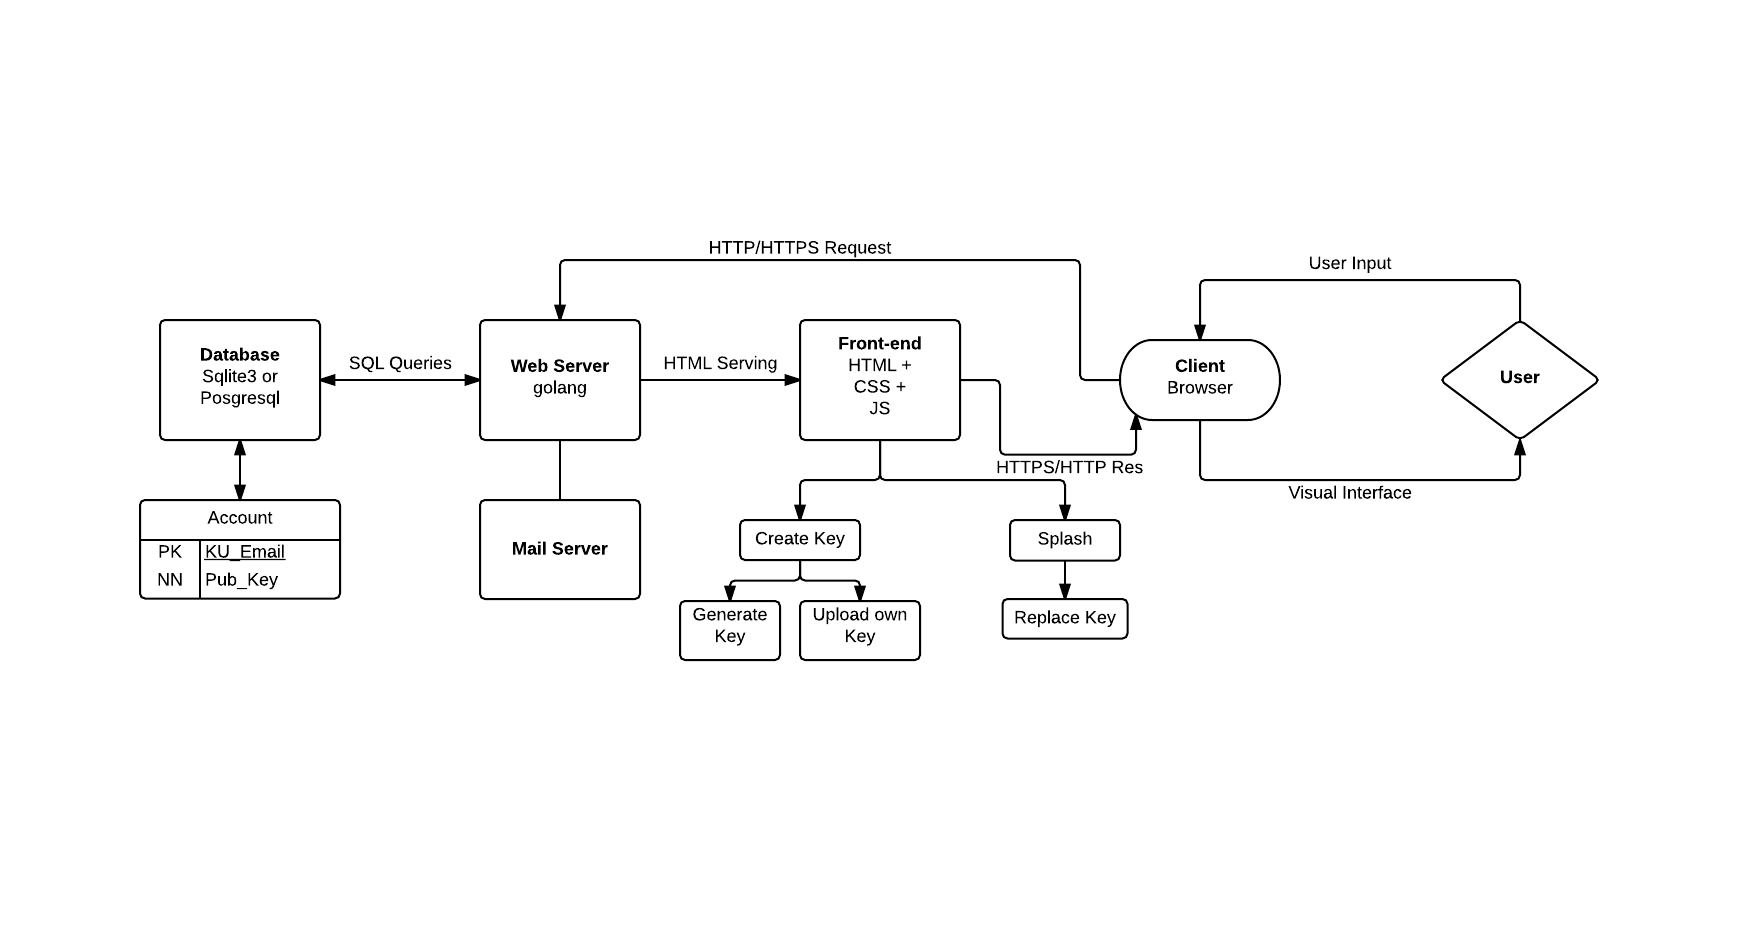
\includegraphics[width=1.1\textwidth]{pictures/pksu_isa_centered.png}
\caption{Initial software architecture of the project. Our project includes coding the database, web server, and front-end.}
\label{fig:ISA}
\end{figure}
\subsection{Project Agreement definition}
\subsection{(e)}
\section{Systemdefintion}
\end{document}
